\documentclass[tikz, margin=5mm]{standalone}

\usetikzlibrary{positioning, shapes.misc}

\begin{document}

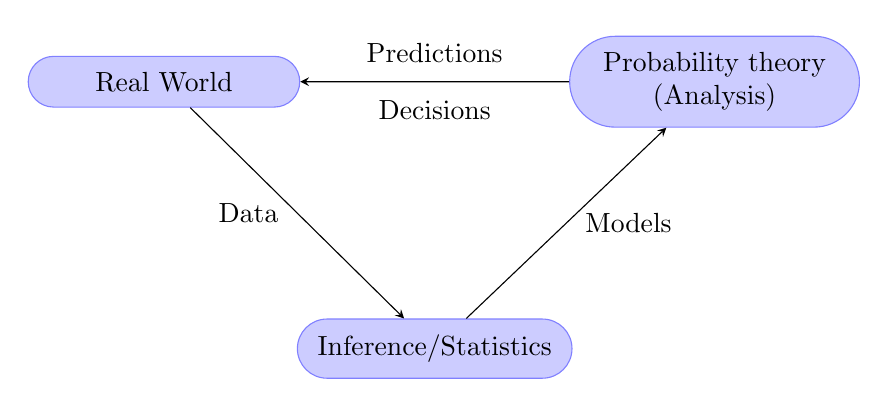
\begin{tikzpicture}
  [>=stealth, inner sep=2mm,
  textbox/.style={fill=blue!20, draw=blue!50, rounded rectangle, text width=3cm, align=center}]
  \draw node at (0,0) (origin) {};
  \draw node (rw) [textbox, left=1.5cm of origin] {Real World};
  \draw node (is) [textbox, below=2.8cm of origin] {Inference/Statistics};
  \draw node (pta) [textbox, right=1.5cm of origin] {Probability theory\\(Analysis)};
  \draw [->] (rw) -- node [left=1pt]{Data} (is);
  \draw [->] (is) -- node [right=1pt]{Models}(pta);
  \draw [->] (pta) -- node [above=1pt]{Predictions} node [below=1pt]{Decisions} (rw);

\end{tikzpicture}
\end{document}